\section{Evaluation}
\label{sec:evalsetup}

We demonstrate the capabilities of our approach by generating test-cases for three different situations:
\begin{enumerate}
\item left turn at a multi-lane 4-way stop,
\item left turn at a T-intersection from the continuing highway to the terminating highway,
\item left turn at a 3-way uncontrolled Y-intersection.
\end{enumerate}
%
For each of these static environments, we generate a sequence of increasingly complex test-cases.
%
The videos and logs of the test-cases, also the traffic rules' encoding in Clingo \cite{Gebser.2018}, are available on the web\footnote{\url{https://www.dropbox.com/sh/e6q4hw98ert5yj7/AAAgo7IlYRKg-rYs7Q9GyMx9a?dl=0}}.
%
The solvability and complexity certificates are visualized in the videos with green and red egos, respectively.


%---executing test-cases
CARLA has several built-in autopilot software that have access to the full simulation state.
%
We subject two specific autopilot agents to the test suite which are automatically generated by our algorithm.
%
We observe that autopilot can fail as we increase the complexity of the test-cases.
%
Finally, we test CARLA's autopilot when  Intel's Responsibility Sensitive Safety (RSS) is added to safeguard autopilot's actions.
%
We observe fewer failures when RSS is enabled, but still autopilot-plus-RSS doesn't pass all the test-cases.


%---the challenge of solving the problem
Our straightforward attempt using Scenic's probabilistic programming failed to find solutions to the search problem.
%
The search space is uncountably infinite so there are too many ways to modify a failed sample.
%
On the other hand, the solution space is highly restricted with continuous and discrete constraints and intertwined dependencies, as explained in the previous section.
%
More specifically, traffic rules depend on only a few discrete events, so they partition the search space into big equivalence classes.
%
Probabilistic mutation of trajectories is searching for a target class by walking within big classes and looking for their boundaries.
%
In contrast, our ASP approach is identifying all the target classes by looking from the above, then searching for a sample within each of them.

\subsection{Results}
We use Scenic \cite{Fremont.2020} as an interface to CARLA to execute a generated test-case, e.g. to test CARLA's autopilot (playing the role of ego).


%---------------------------------------
\begin{figure}[ht]% >>>
  \centering
  \begin{minipage}[t]{.499\linewidth}
    {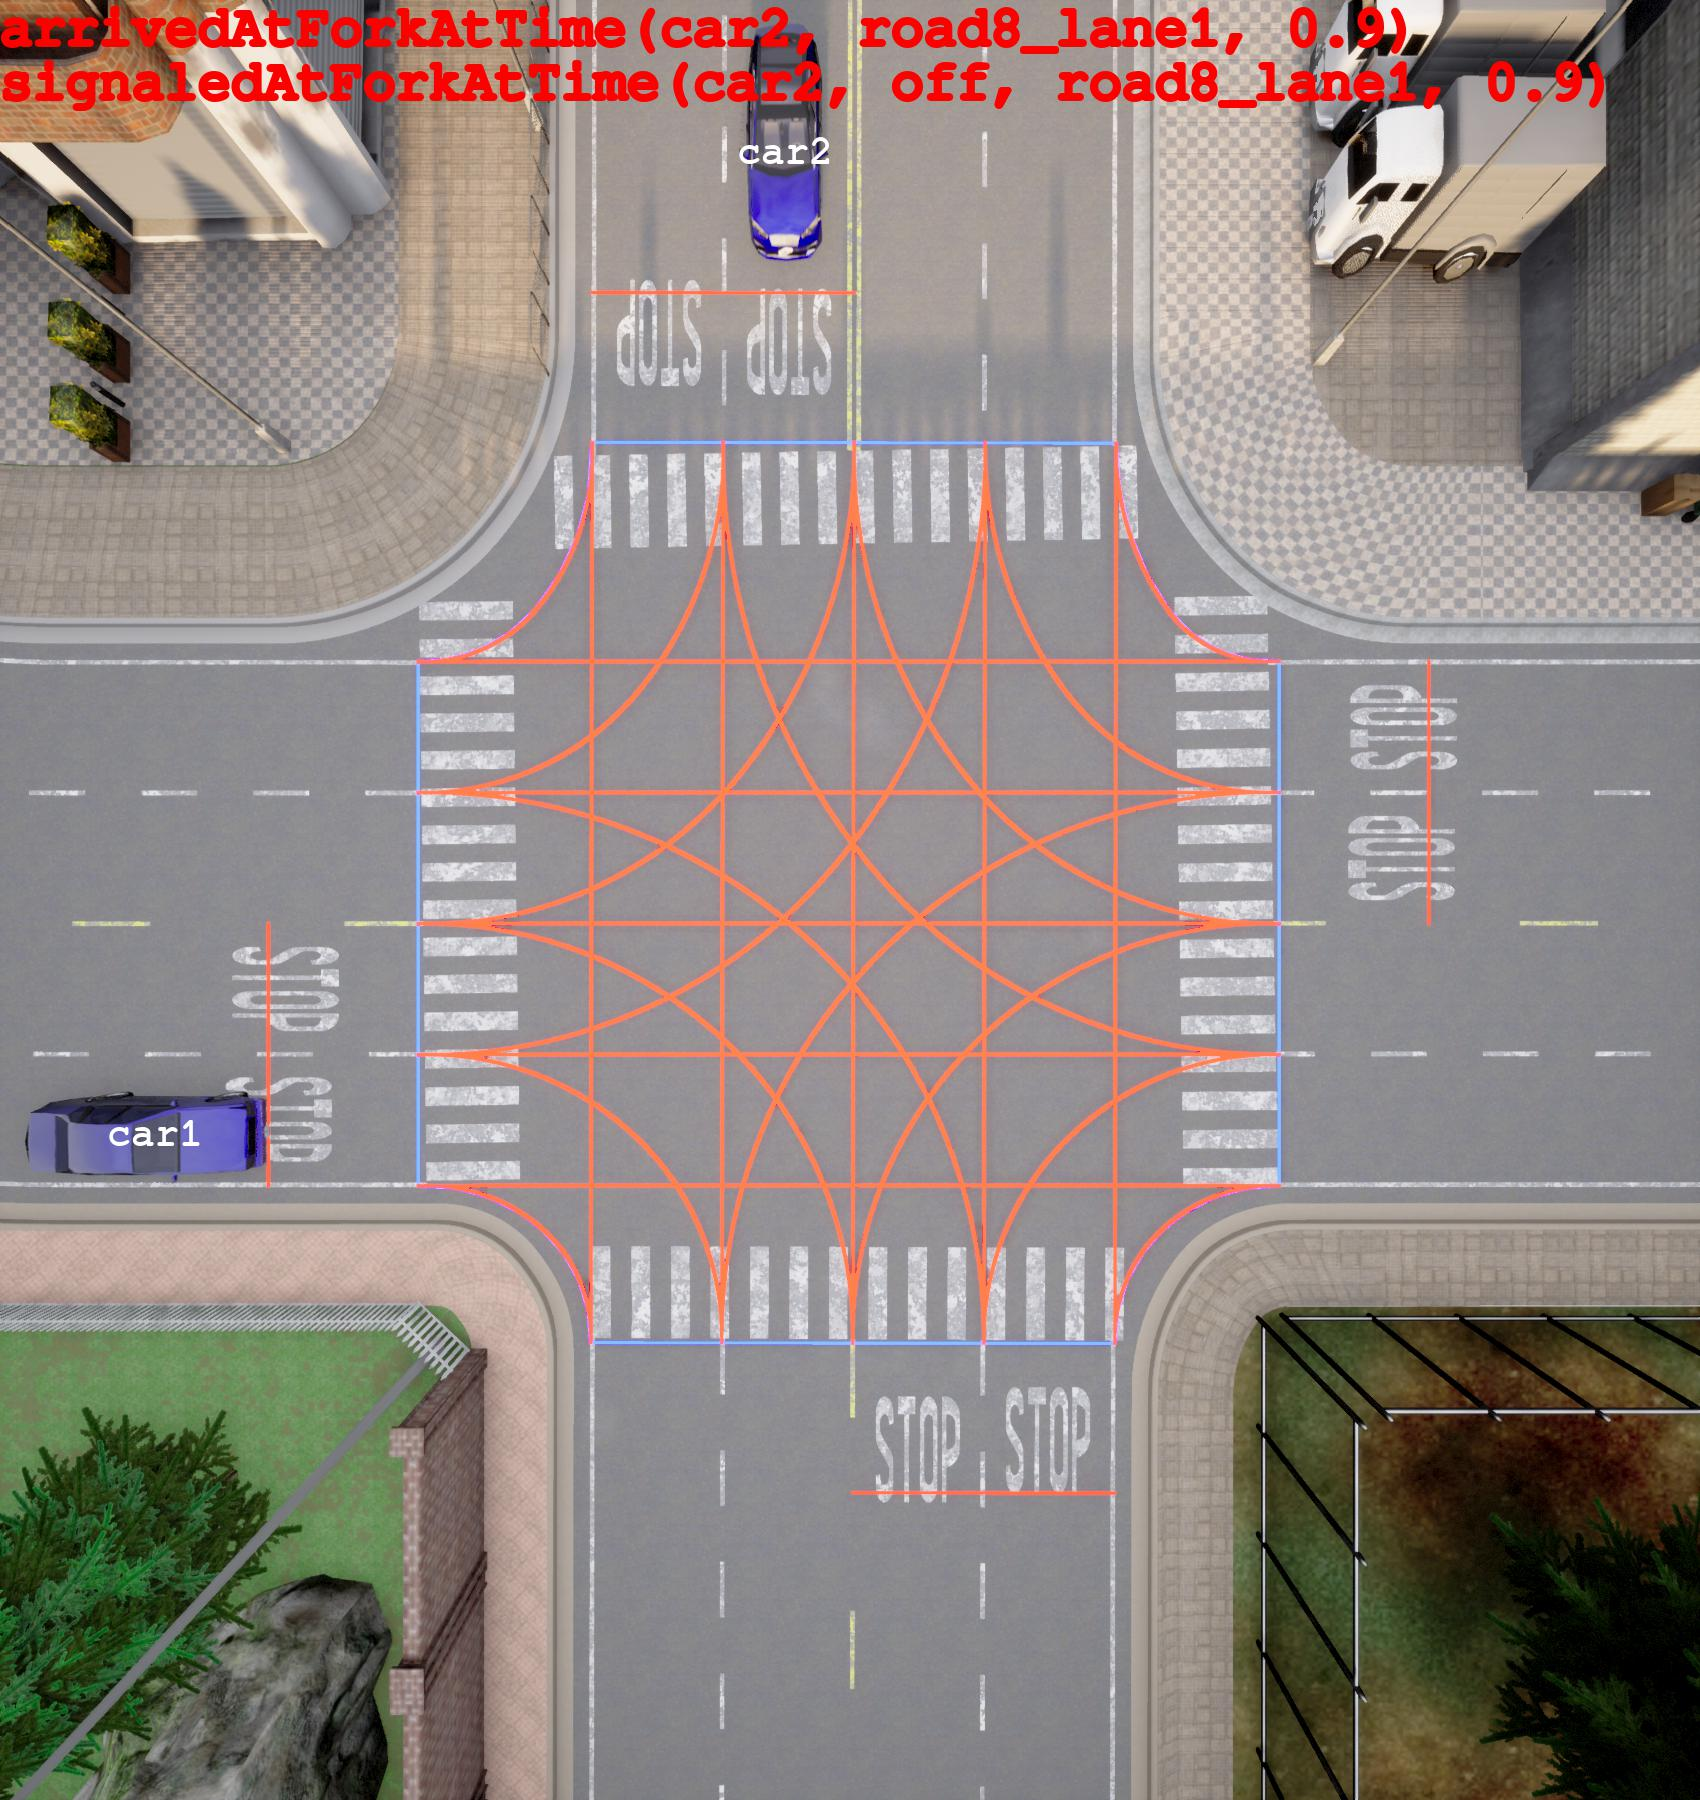
\includegraphics[width=\linewidth]{figures/chapter4/2_18.jpg}}%
    \subcaption{car2 arrives.}
  \end{minipage}%
  \hfill
  \begin{minipage}[t]{.499\linewidth}
    {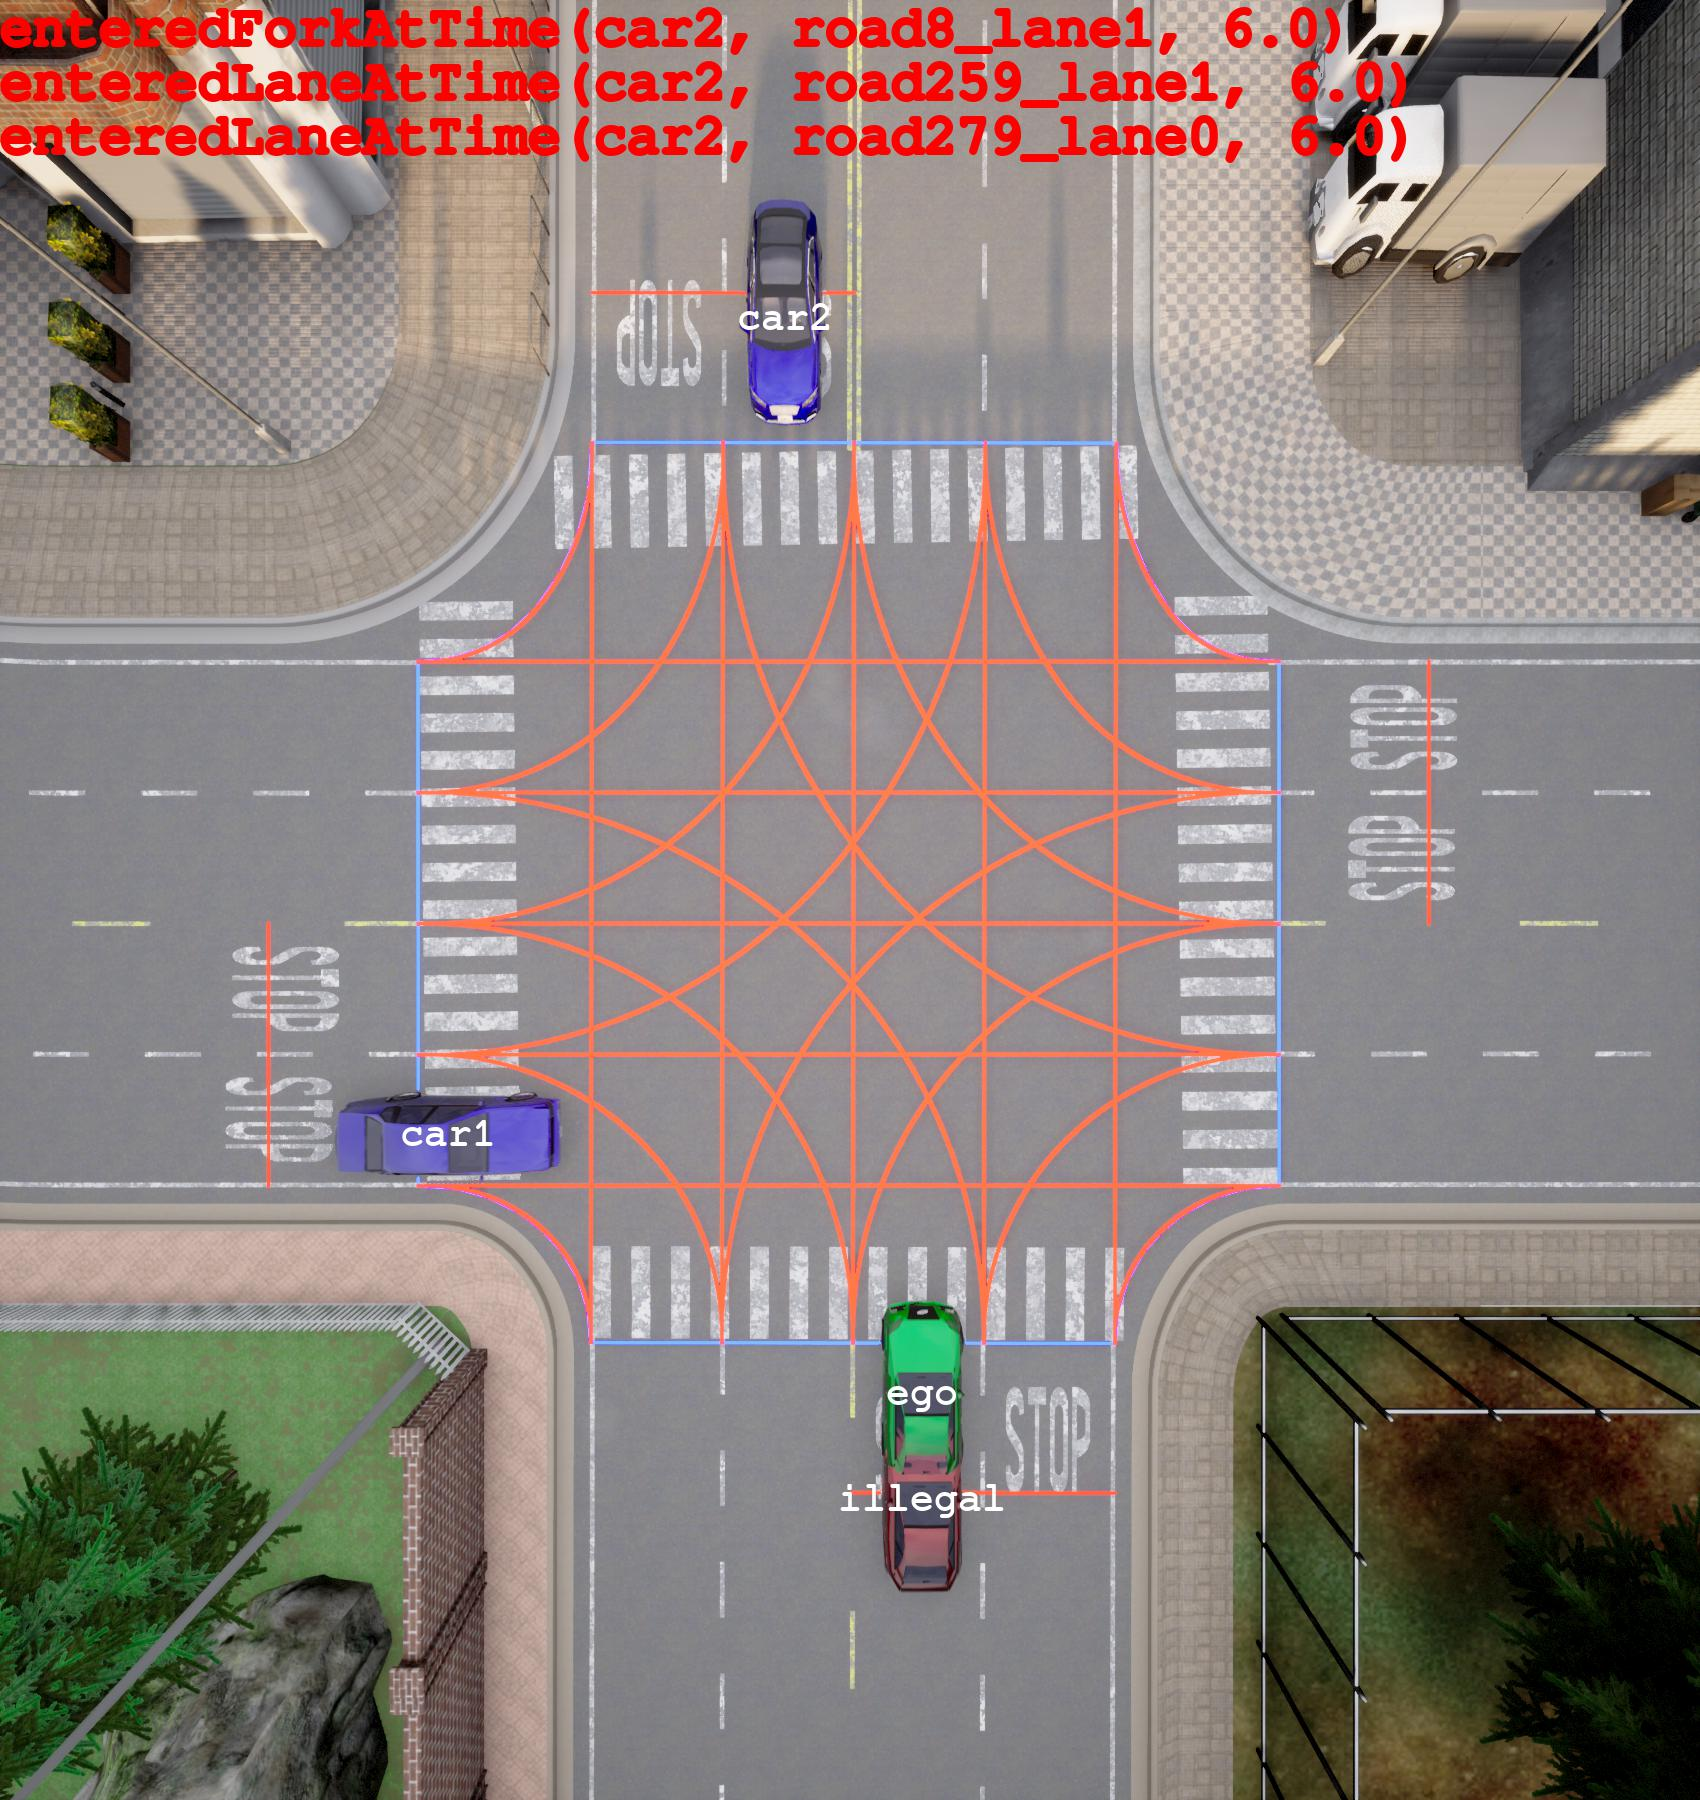
\includegraphics[width=\linewidth]{figures/chapter4/2_120.jpg}}%
    \subcaption{car2 enters.}
  \end{minipage}%
  \hfill
  \begin{minipage}[t]{.499\linewidth}
    {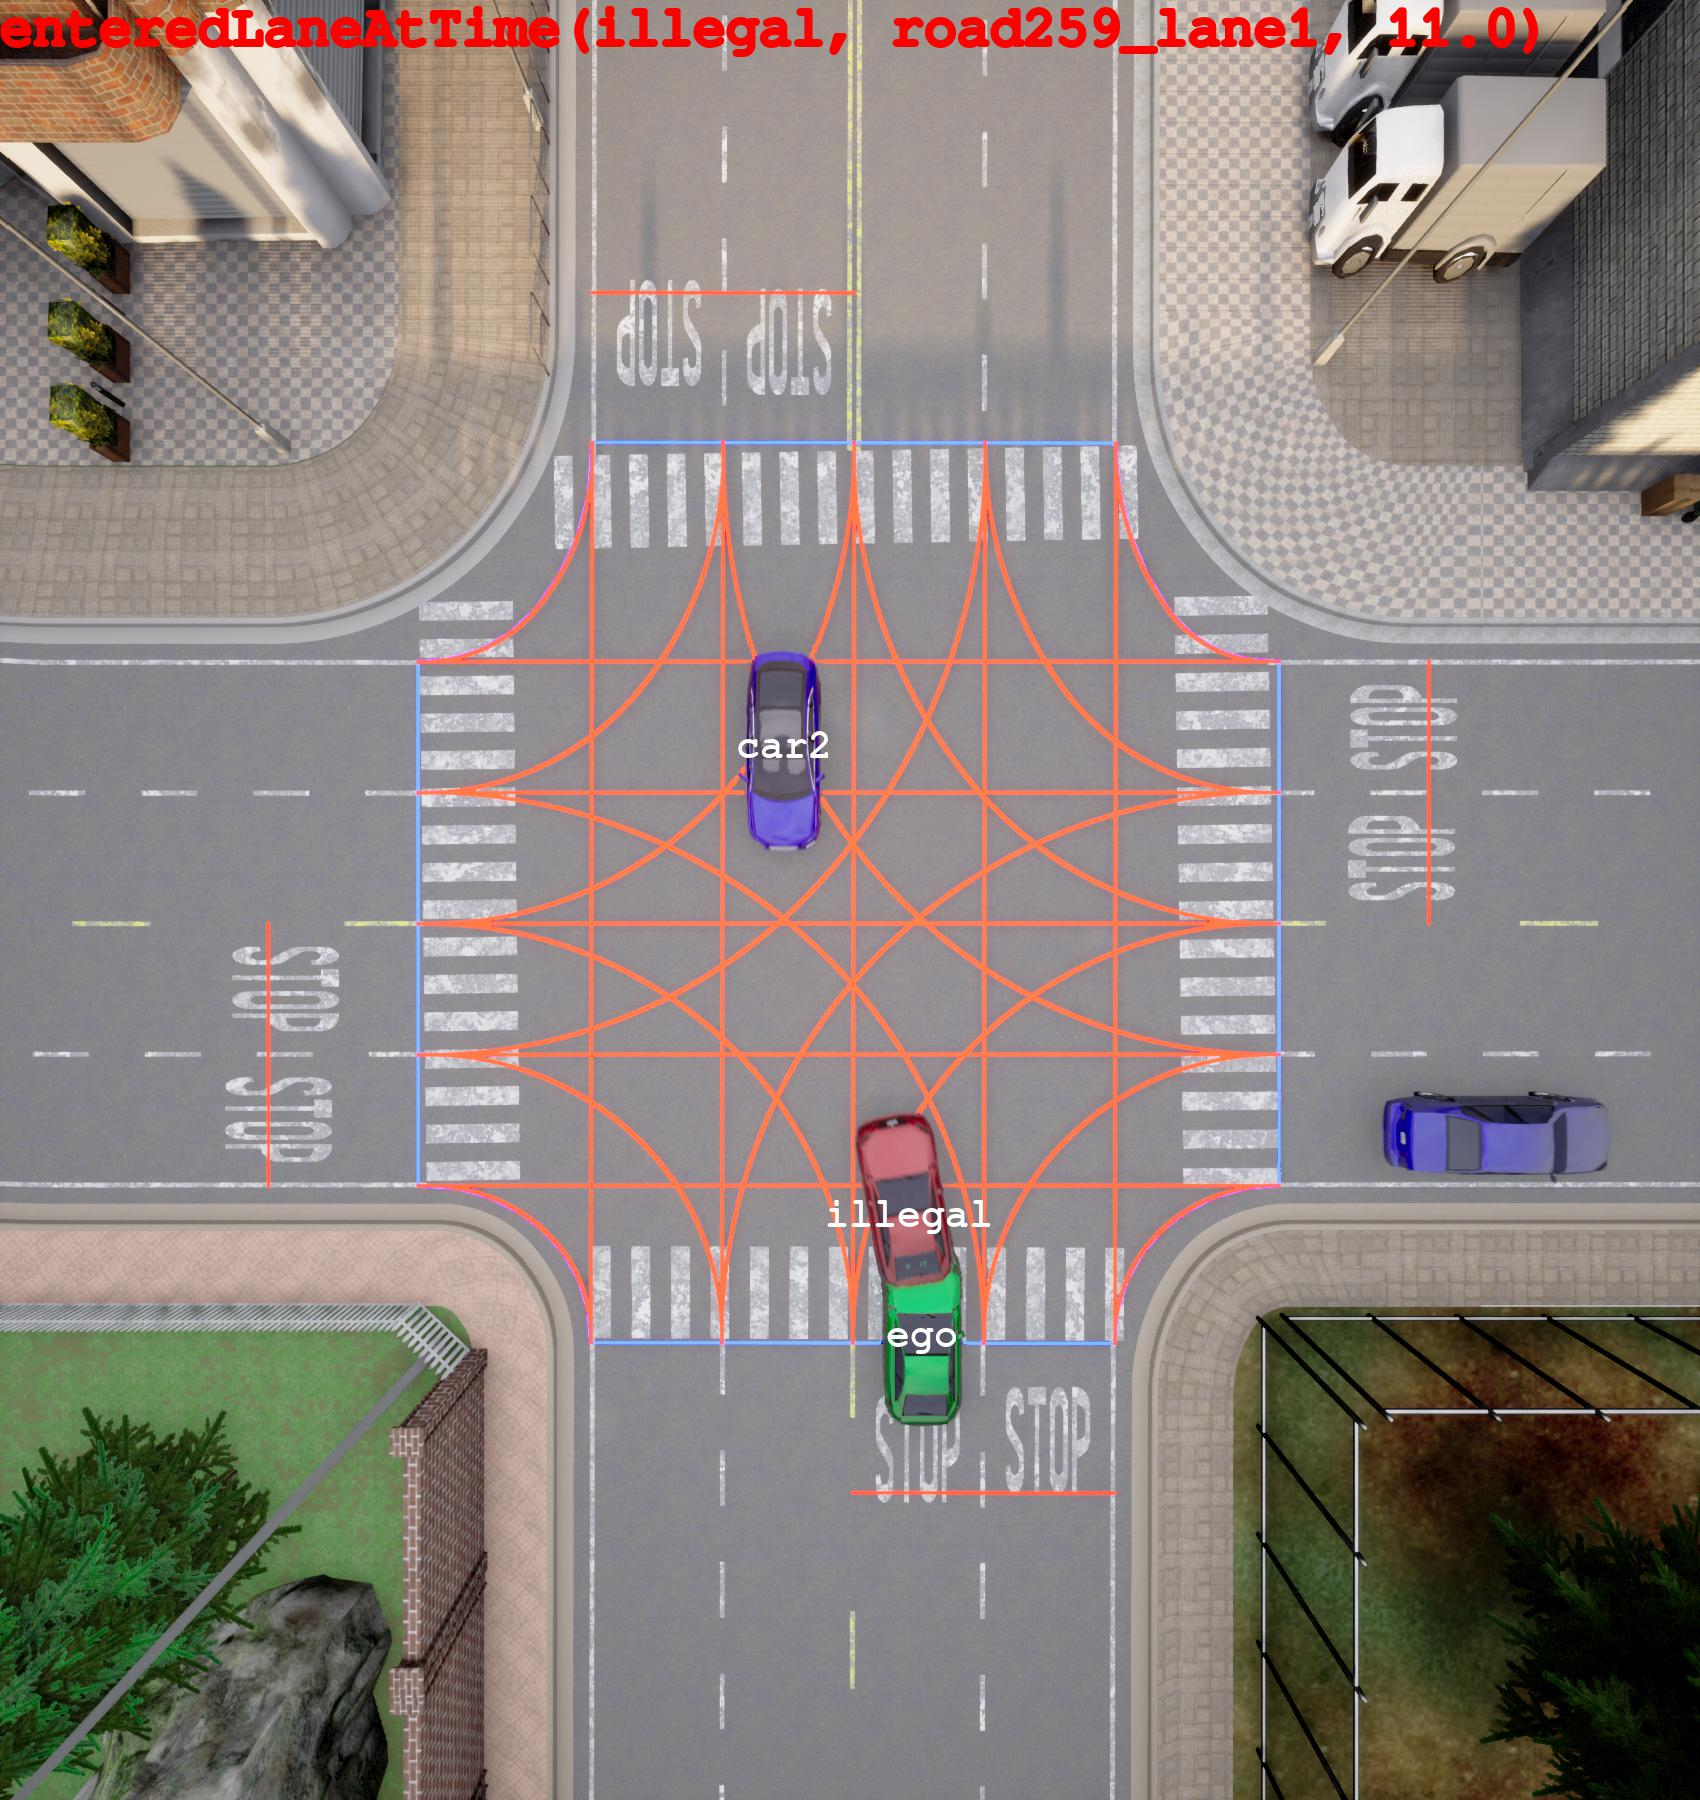
\includegraphics[width=\linewidth]{figures/chapter4/2_220.jpg}}%
    \subcaption{illegal enters car2's route.}
  \end{minipage}%
  \hfill
  \begin{minipage}[t]{.499\linewidth}
    {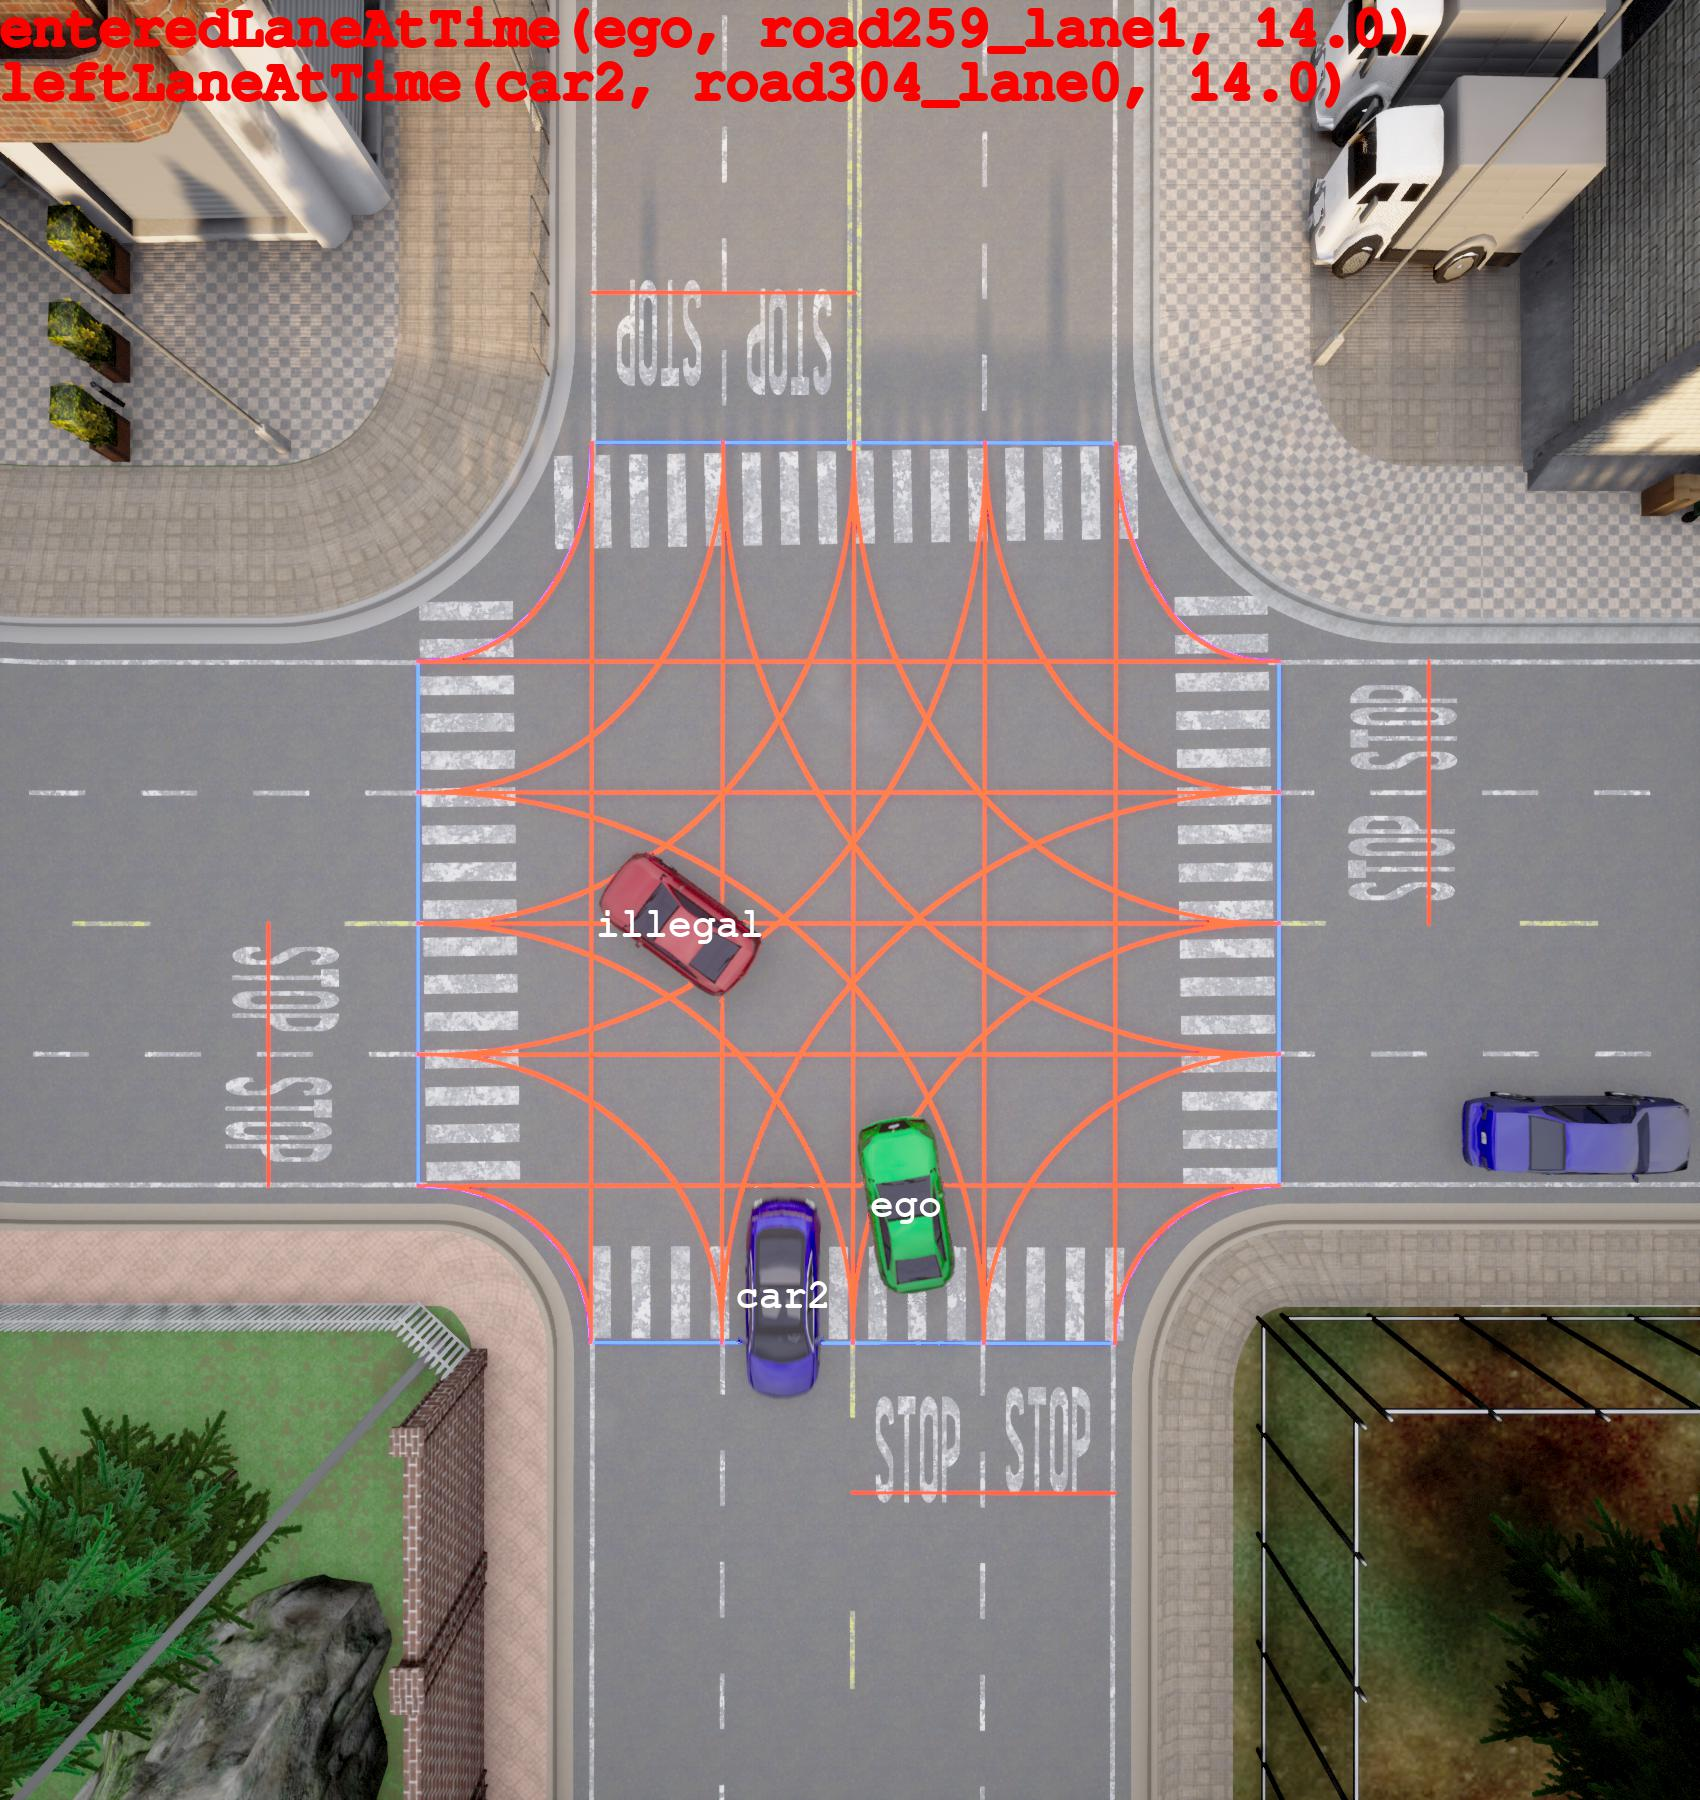
\includegraphics[width=\linewidth]{figures/chapter4/2_280.jpg}}%
    \subcaption{ego enters car2's route.}
  \end{minipage}%
  \caption{Left turn from a 4way-stop.}
  \label{fig:4way}%
\end{figure}% <<<

\textbf{Four-way Stop:} The first example demonstrates making incrementally more complex test-cases by adding more non-egos.
%
The goal of ego is to make a left turn from a four-way stop.
%
Ego starts from the bottom side of the intersection in Figure~\ref{fig:4way} and must exit the intersection from the left side.
%
We generate three test-cases, each more complex than the previous one.
%
In the first test-case a non-ego is added that enters the intersection from the left and passes straight through the intersection.
%
In the second test-case (visualized in Figure~\ref{fig:4way}), a non-ego is added that approaches from the top, the opposite side of ego, and passes straight through the intersection.
%
In the third test-case, a non-ego is added that approaches also from the left but the other lane of the road, and passes straight through the intersection.
%
Both CARLA's autopilot and autopilot-plus-RSS pass the first test-case.
%
Autopilot fails the second test-case while autopilot-plus-RSS passes it.
%
Finally, both autopilot and autopilot-plus-RSS fail the third test-case.
%
See the videos for even more complex extensions of this test-case.


%---------------------------------------
\begin{figure}% >>>
  \centering
  \begin{minipage}[t]{.499\linewidth}
    {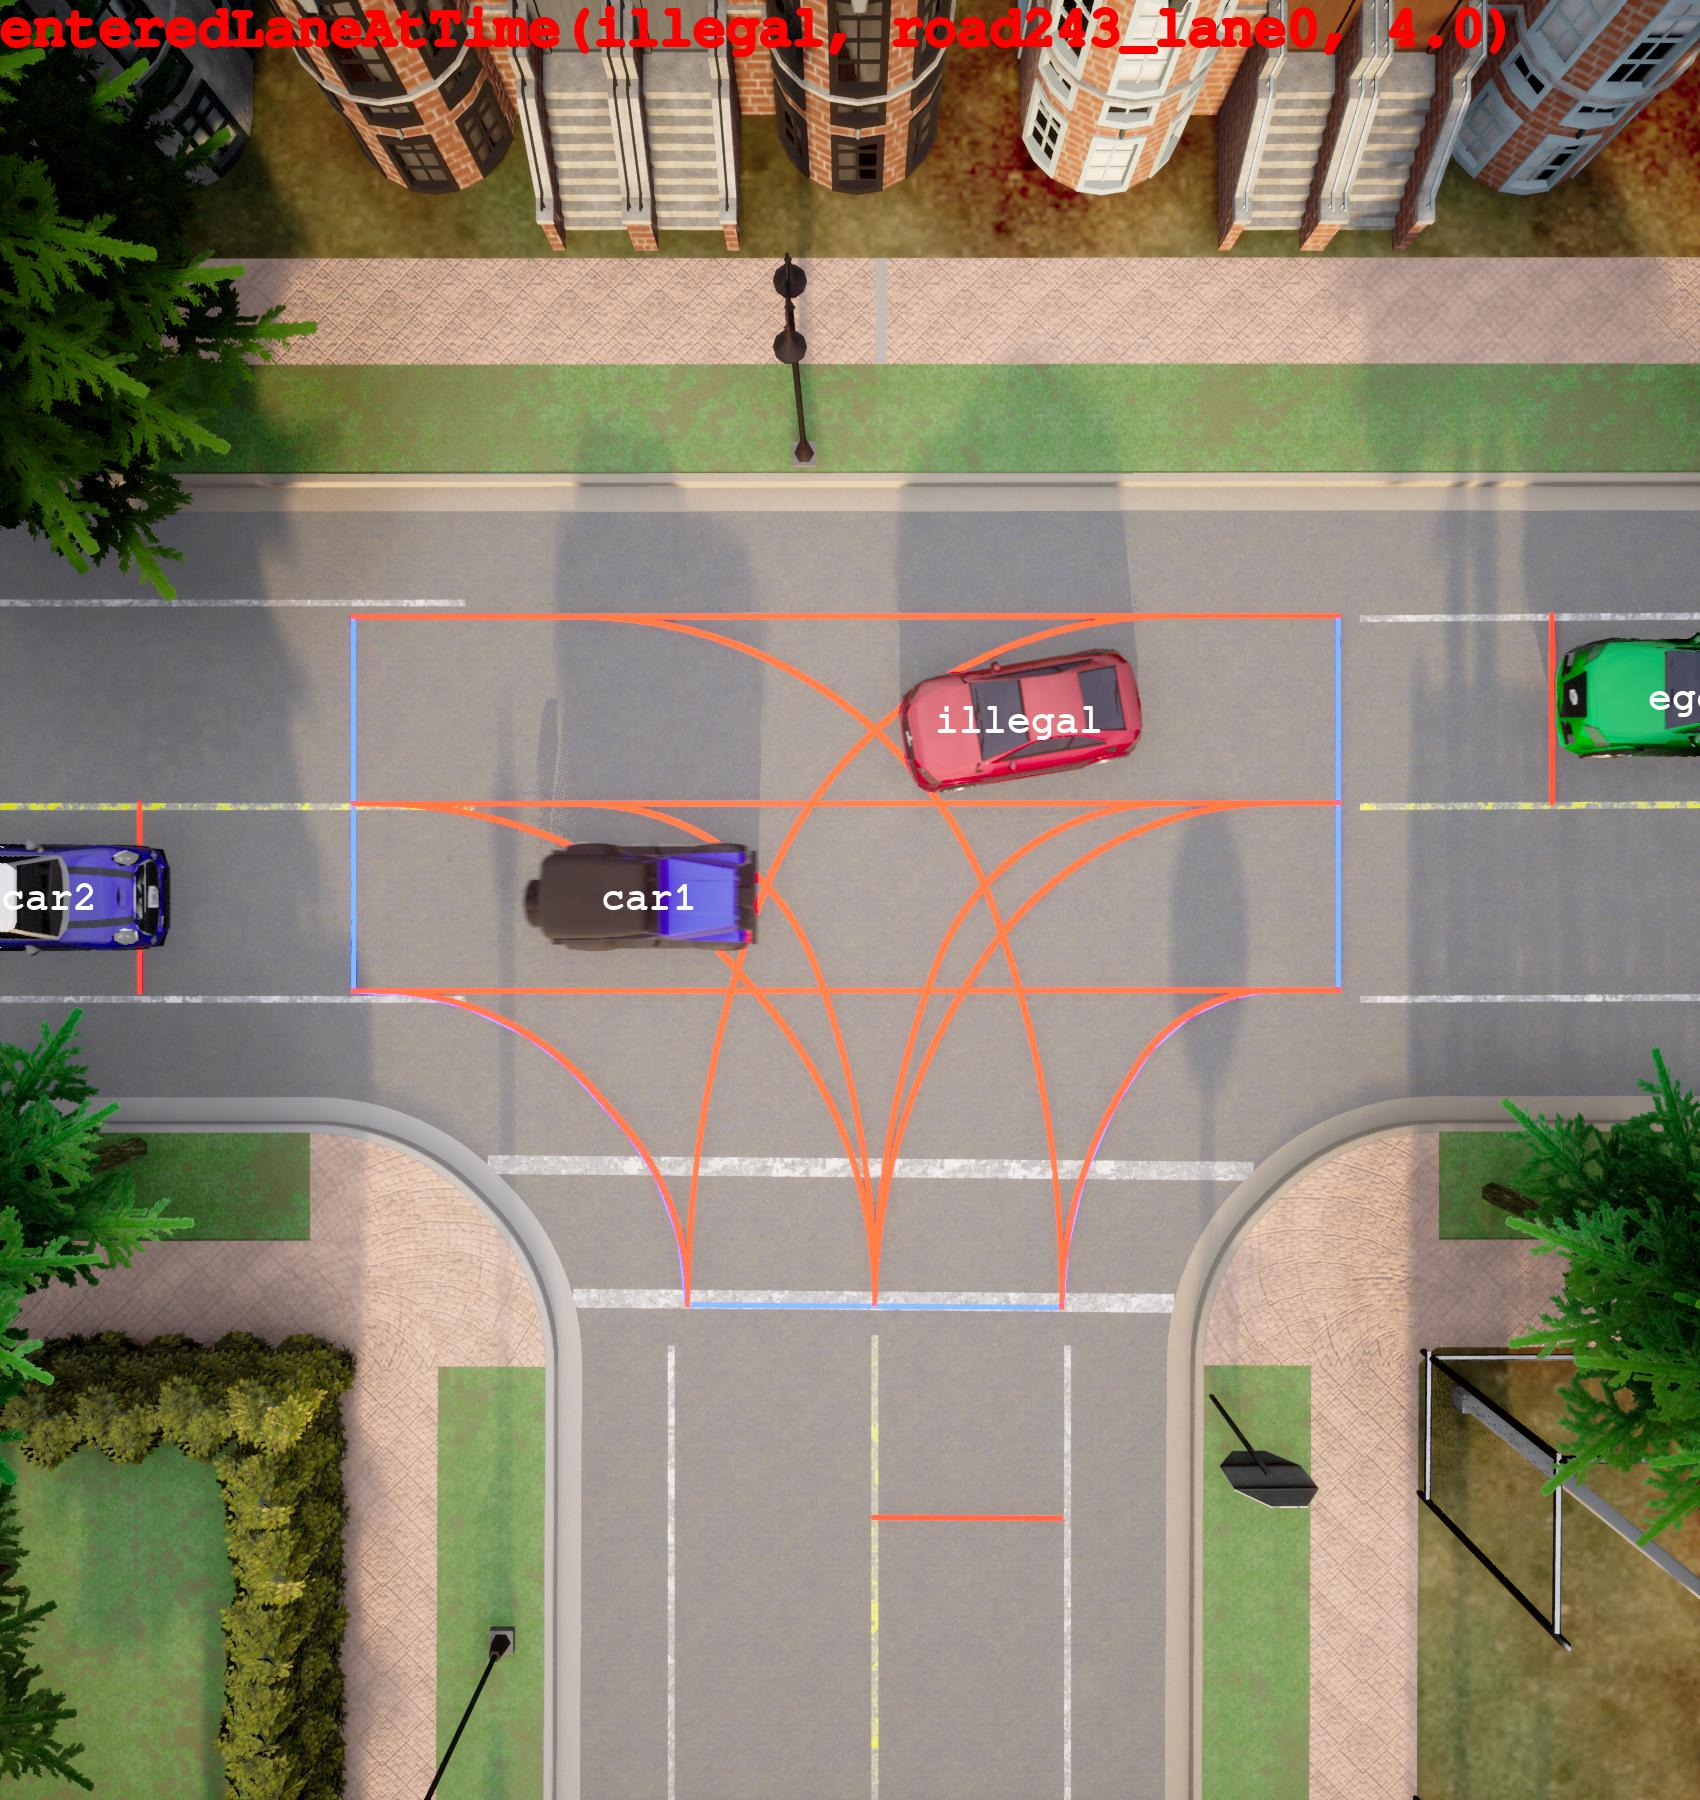
\includegraphics[width=\linewidth]{figures/chapter4/T-intersection/1_80.jpg}}%
    \subcaption{car2 approaches (passes the red line) before illegal enters car2's route}
  \end{minipage}%
  \hfill
  \begin{minipage}[t]{.499\linewidth}
    {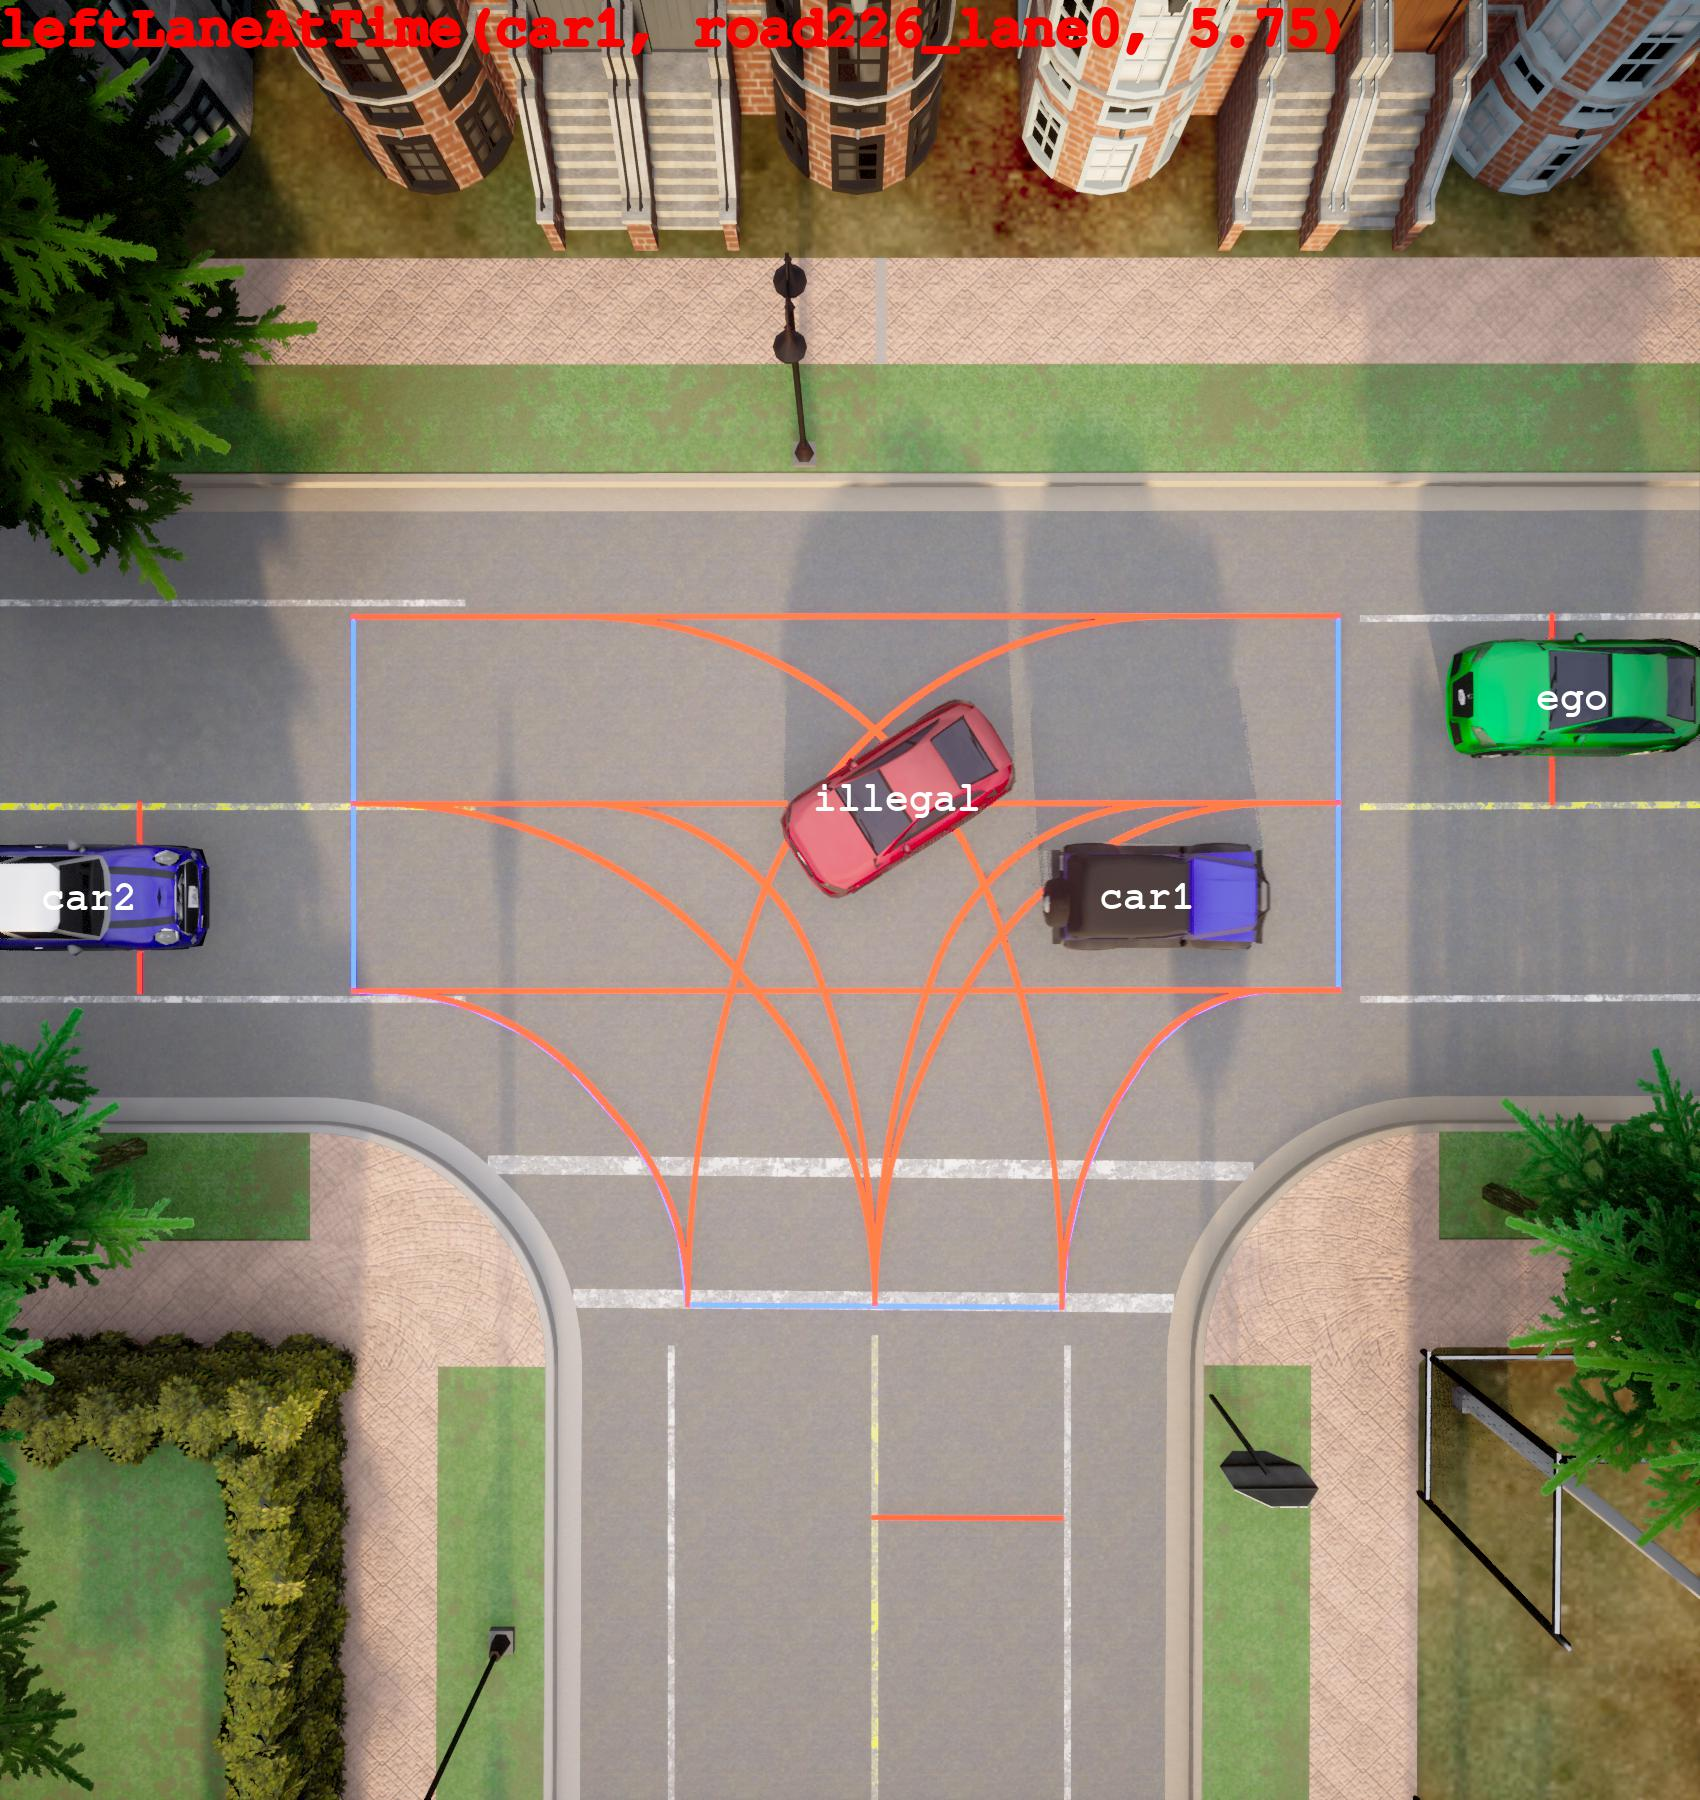
\includegraphics[width=\linewidth]{figures/chapter4/T-intersection/1_115.jpg}}%
    \subcaption{illegal does not yield to car2}
  \end{minipage}%
  \caption{Unprotected left turn from continuing highway.}\label{fig:continuing}%
\end{figure}% <<<


\textbf{T-intersection:} The goal of ego is to perform an unprotected left turn from the continuing highway to the terminating highway of the T-intersection shown in Figure \ref{fig:continuing}.
%
Ego approaches the intersection from the right side and must make a left turn to enter the road on the bottom.
%
This example demonstrates that we can add multiple non-egos to a test-case simultaneously.
%
Starting with an empty test-case, our test-case generator adds multiple non-egos that pass straight through the intersection from left to right.
%
CARLA's autopilot fails this test-case but autopilot-plus-RSS passes it.



%-------------------------------------------------------
\begin{figure}[ht]% >>>
  \centering
  \begin{minipage}[t]{.499\linewidth}
    {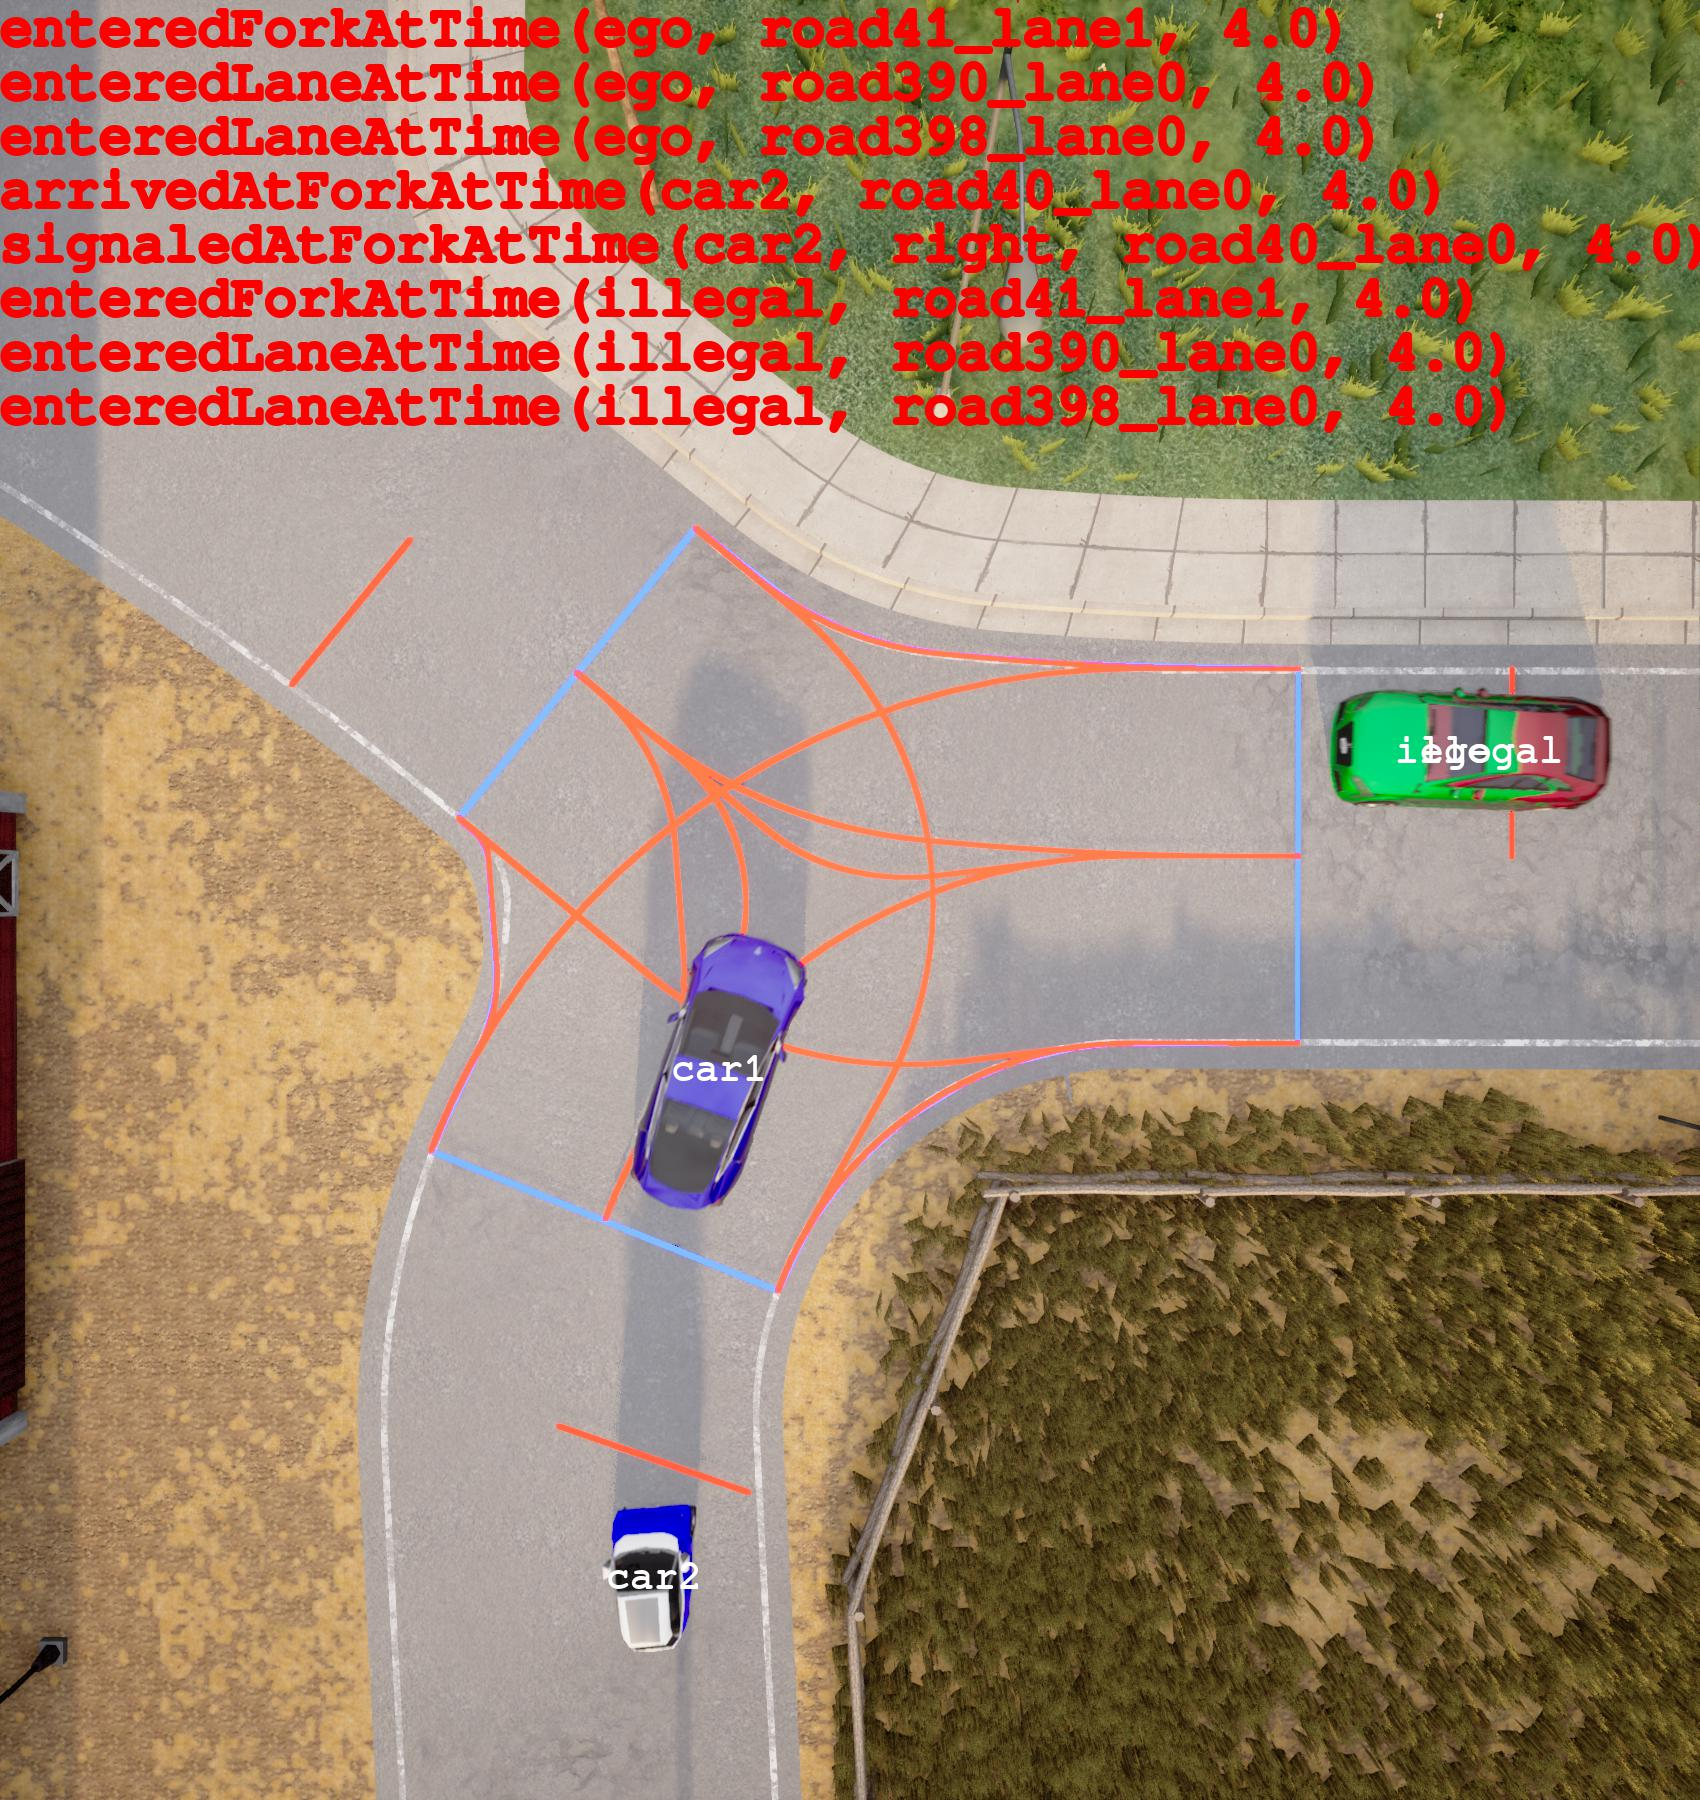
\includegraphics[width=\linewidth]{figures/chapter4/Y-intersection/1_80.jpg}}%
    \subcaption{car1 enters earlier than ego and illegal.}
  \end{minipage}%
  \hfill
  \begin{minipage}[t]{.499\linewidth}
    {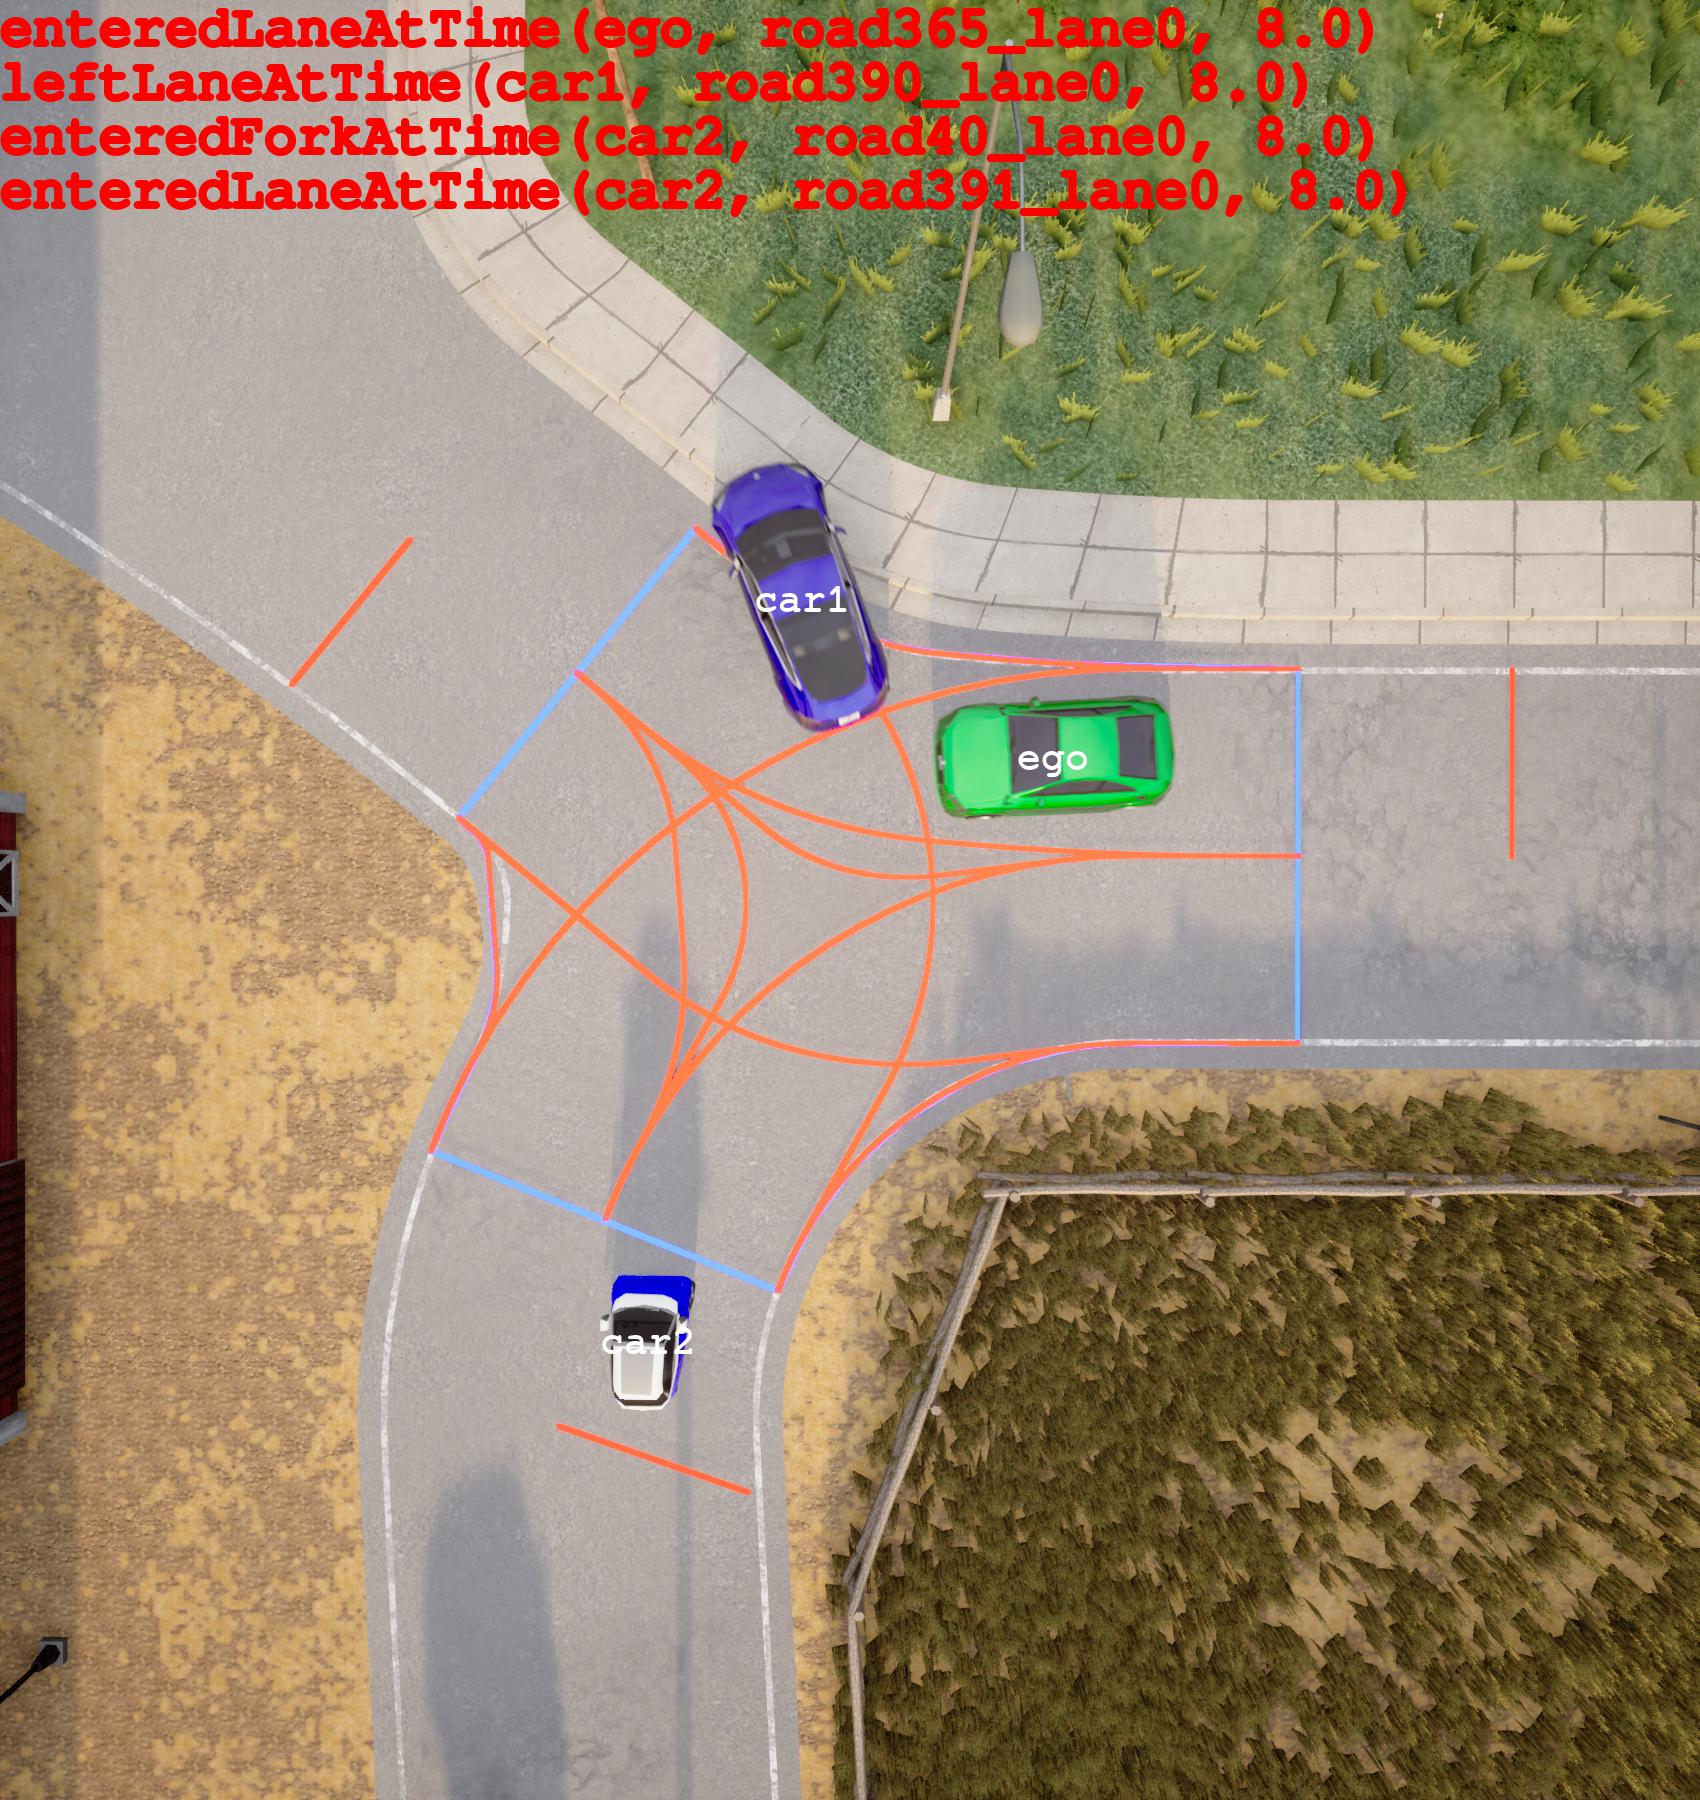
\includegraphics[width=\linewidth]{figures/chapter4/Y-intersection/1_160.jpg}}%
    \subcaption{illegal already exited from the bottom but ego waited for car1.}
  \end{minipage}%
  \caption{Unprotected left turn from an uncontrolled Y-intersection.}\label{fig:Y-intersection}%
\end{figure}% <<<


\textbf{Y-intersection:} The third example demonstrates that we can add a non-ego whose route does not conflict ego's route, as long as we add also a non-ego whose route has a conflict so that the test-case can become more complex.
%
Autopilot fails this test-case.
%
Running Autopilot-plus-RSS results in a segmentation fault which seems to be due to a bug in CARLA's map or integration of RSS.
%
Ego's goal is to approach from right and make a left turn to the bottom of the intersection.
%
The conflicting non-ego, {\verb car1 }, approaches from the bottom, makes a left turn and exits from the top left corner of the intersection.
%
The non-conflicting non-ego, {\verb car2 }, also approaches from the bottom, but makes a right turn and exits from the right side of the intersection.

